\section{Architecture} \label{sec:raftian}

In the previous section (\ref{sec:raft}) we explained in detail how nodes communicate with each other and handle their log. Now we will explain what actually happens inside a node. Before showcasing the architecture, we will briefly explain how Pygame works, and thus take the opportunity to present the user interface.

\subsection{Pygame} 

Pygame's approach is very straightforward: first comes the declaration and set up of all the graphical components, such as game window, fonts, colors, variables and constants. Every element gets positioned on the main window by coordinates \textit{(x,y)}, where \textit{(0,0)} is the top left corner. Most items are made of two fundamental Pygame classes: \textit{Rect}, which creates non-graphical objects that expose many useful methods, for example to position, move, and resize themselves, or to detect collisions and mouse clicks, and \textit{Surface}, which is the most basic graphical component that has dimensions and can be drawn upon. Often we want to bind, thus constrain, surfaces with rects so that we use the latter for spatial operations. One last fundamental is the \textit{blit} function, a method that draws one image onto another or, to be precise, that draws a source Surface onto the object Surface that calls it. We can give it an optional argument to specify a drawing destination, either with coordinates or a rect. To clarify: $baseSurface.blit(sourceSurface,destination)$ draws \textit{sourceSurface} onto \textit{baseSurface} at the coordinates specified by \textit{destination}. An example of all the above can be seen at listing \ref{code:pygameIntro}.

Pygame, being low-level in nature, grants us great flexibility, allowing us to do pretty much whatever we want. For example, we defined our players as dataclasses that encapsulate both the players' data (like \textit{id} or \textit{health points}) and their Rect and Surface objects. An example can be seen at listing \ref{code:pygamePlayer}.

Finally, Pygame gives us direct access to the game loop, which is implemented as nothing more than a \textit{while loop}. In it, we can process player inputs and refresh the screen, dynamically changing what gets shown. In short, we manage everything that happens while the game is running. In listing \ref{code:pygameLoop} we can see two types of player input, one for quitting the game and a left-mouse click, the latter of which causes a refresh of the header. Specifically, if \textit{Player 2} gets clicked, the header will display \textit{"Player 2 pressed"}, reverting back to its original state after a couple of seconds. The last command, \textit{clock.tick(fps)}, allows us to limit the framerate, effectively slowing down or speeding up the game engine itself by constraining the amount of times per second the game loop repeats itself.

\begin{python}[label={code:pygameIntro}, caption={Pygame base components}]
pygame.init()                                   # starts pygame
GREY = (125, 125, 125)                          # define a color
DISPLAY = pygame.display.set_mode((1000, 1200)) # creates game window 1000x1200 pixels in resolution
clock = pygame.time.Clock()                     # necessary to mange fps
font = pygame.font.Font(None, 60)               # creates default font 
toptext = font.render("Top Text", False, BLACK) # header text
rect_header = pygame.Rect(0, 0, 1000, 100)      # creates rect for header
header = pygame.Surface((1000, 100))            # creates surface for header
header.fill(WHITE)                              # draw on surface 

DISPLAY.blit(header, rect_header)               # draw on DISPLAY the header surface
                                                # position is given by rect_header                                    
#...
# draw text on coordinates
DISPLAY.blit(toptext, (rect_header.centerx - xoffset, rect_header.centery - yoffset))
\end{python}

\begin{python}[label={code:pygamePlayer}, caption={Players defined as dataclassess that encapsulate Pygame elements}]
@dataclass
class Player:
    id: int
    hp: int
    rc: pygame.Rect     # represent player position and size 
    ui: pygame.Surface  # expose UI of the player e.g., colour 

player1 = Player(
    id=1,
    hp=100,
    rc=pygame.Rect(585, 685, 80, 80),  # x0, y0, width, height
    ui=pygame.Surface((80,80))
)
player1.ui.fill(RED)                    # colour player red
DISPLAY.blit(player1.ui, player1.rc)    # draw on display via rect
\end{python}

\begin{python}[label={code:pygameLoop}, caption={All interactions and frame-by-frame rendering happen in the game loop}]
while True: # game loop
    for event in pygame.event.get():    # process player inputs
        if event.type == pygame.QUIT:
            pygame.quit()

        if event.type == pygame.MOUSEBUTTONDOWN and event.button == 1:  # left mouse button click

            pos = pygame.mouse.get_pos() # gets mouse position

            if player.rc.collidepoint(pos): # rect allows us to detect collisions
                toptext = font.render(f"Player {player.id} pressed", False, BLACK)

                DISPLAY.blit(header, rect_header)   # erase previous text
                DISPLAY.blit(toptext, (rect_header.centerx - xoffset, rect_header.centery - yoffset))

    pygame.display.flip()  # refresh on-screen display
    clock.tick(60)         # limits framerate
\end{python}

\subsection{Raftian User Interface}

Figure \ref{fig:raftianUI} shows different phases of a normal Raftian's game session. Specifically, they demonstrate how the interface changes when the player repeatedly click on (thus \textit{attack}) Player 3, the blue one on the top left. Players' colours become progressively desaturated as their health points decrease, by modifying their alpha channels as shown in listing \ref{code:pygamePlayerDamage}. When a player is dead, its colour change to a darker shade. 

On the header an attack message gets written, reverting back after half a second. Said message changes depending whether the player is still alive; if not, damage is ignored. 

\begin{python}[label={code:pygamePlayerDamage}, caption={Whenever a player gets damaged, its colour gets desaturated}]
for player in players:
    if player.id == order.command and player.hp > 0:
        player.hp -= 30  # apply damage to player:

        if player.hp < 90 and player.hp >= 60:
            player.ui.set_alpha(190)
            DISPLAY.blit(player_UI_cleaner, player.rc)  # clean player UI
            DISPLAY.blit(player.ui, player.rc)          # redraw player UI
\end{python}

\begin{figure}[h]
    \centering
    \begin{subfigure}{0.31\textwidth}
        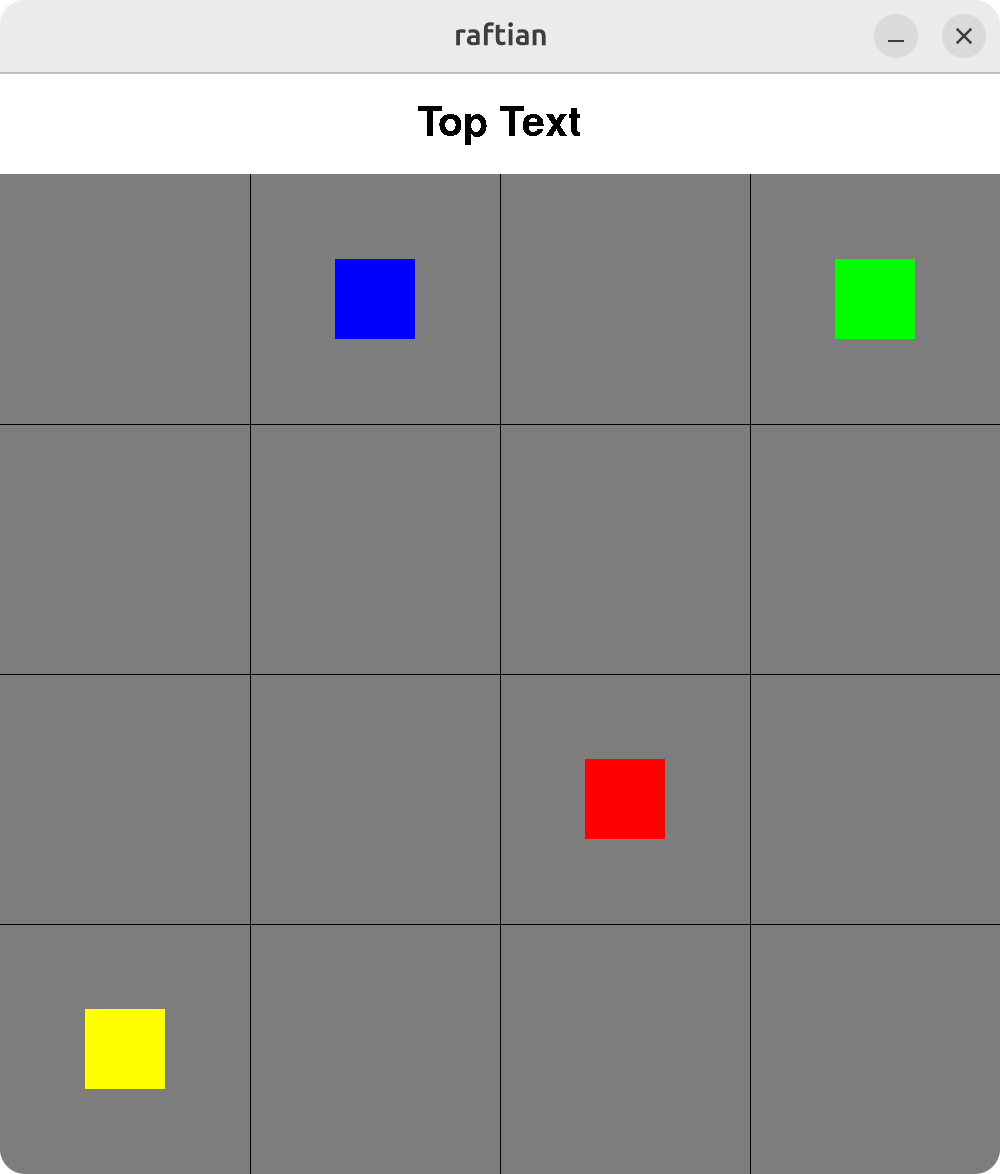
\includegraphics[width=\linewidth]{images/raftian1.png}
        \caption{Game starts}
    \end{subfigure}
    \hfill
    \begin{subfigure}{0.31\textwidth}
        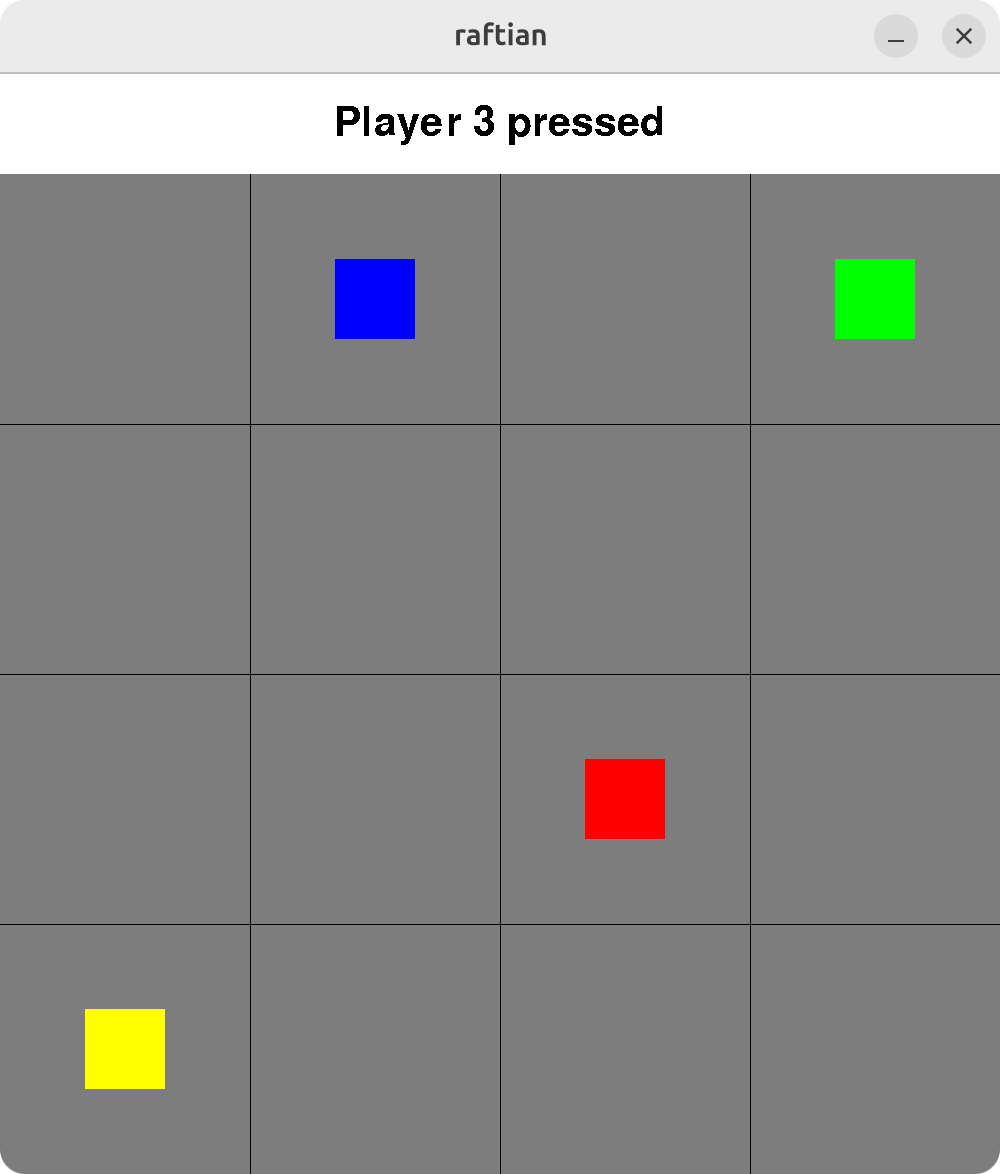
\includegraphics[width=\linewidth]{images/raftian2.png}
        \caption{Player 3 is attacked}
    \end{subfigure}
    \hfill
    \begin{subfigure}{0.31\textwidth}
        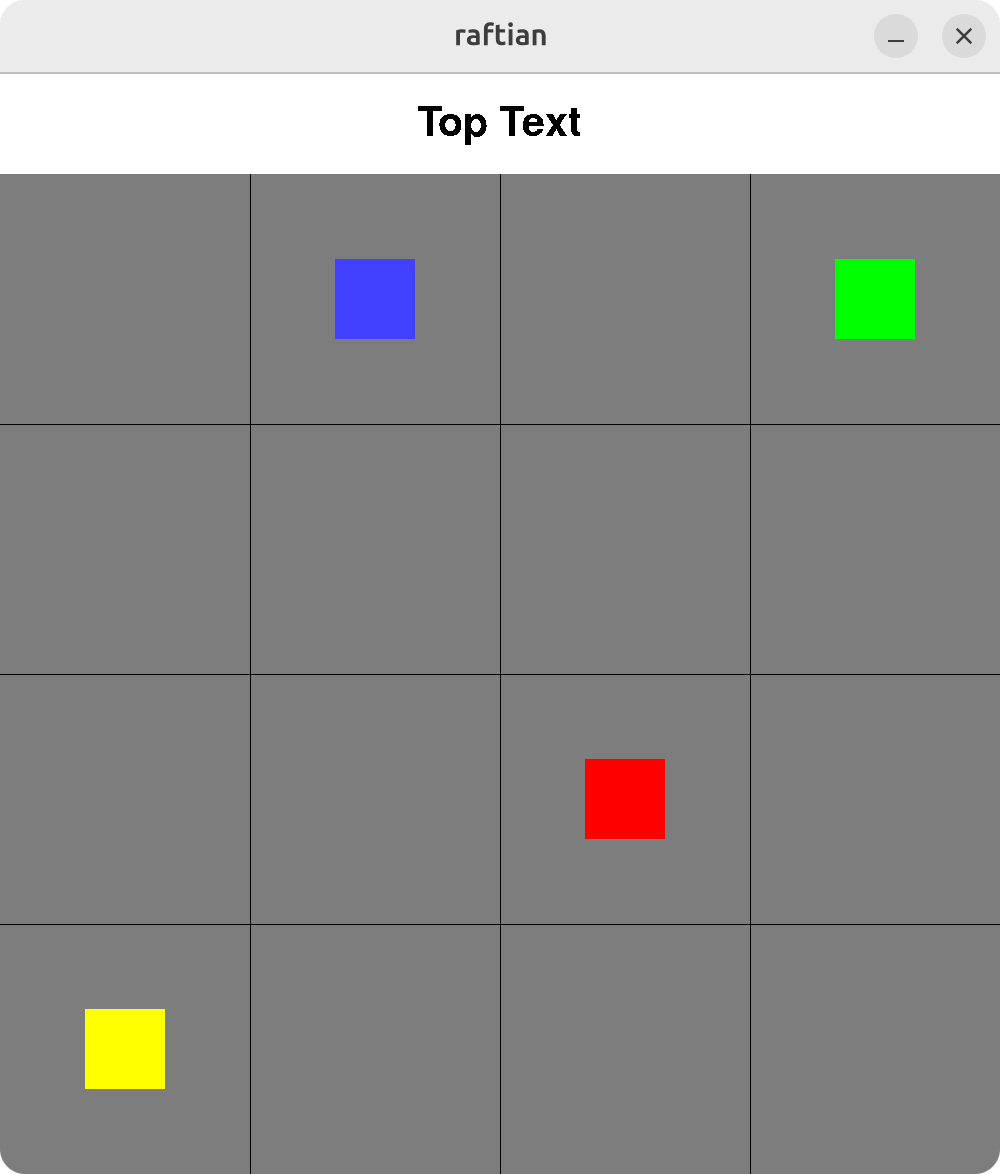
\includegraphics[width=\linewidth]{images/raftian3.png}
        \caption{Header reverts to default}
    \end{subfigure}
    \hfill
    \begin{subfigure}{0.31\textwidth}
        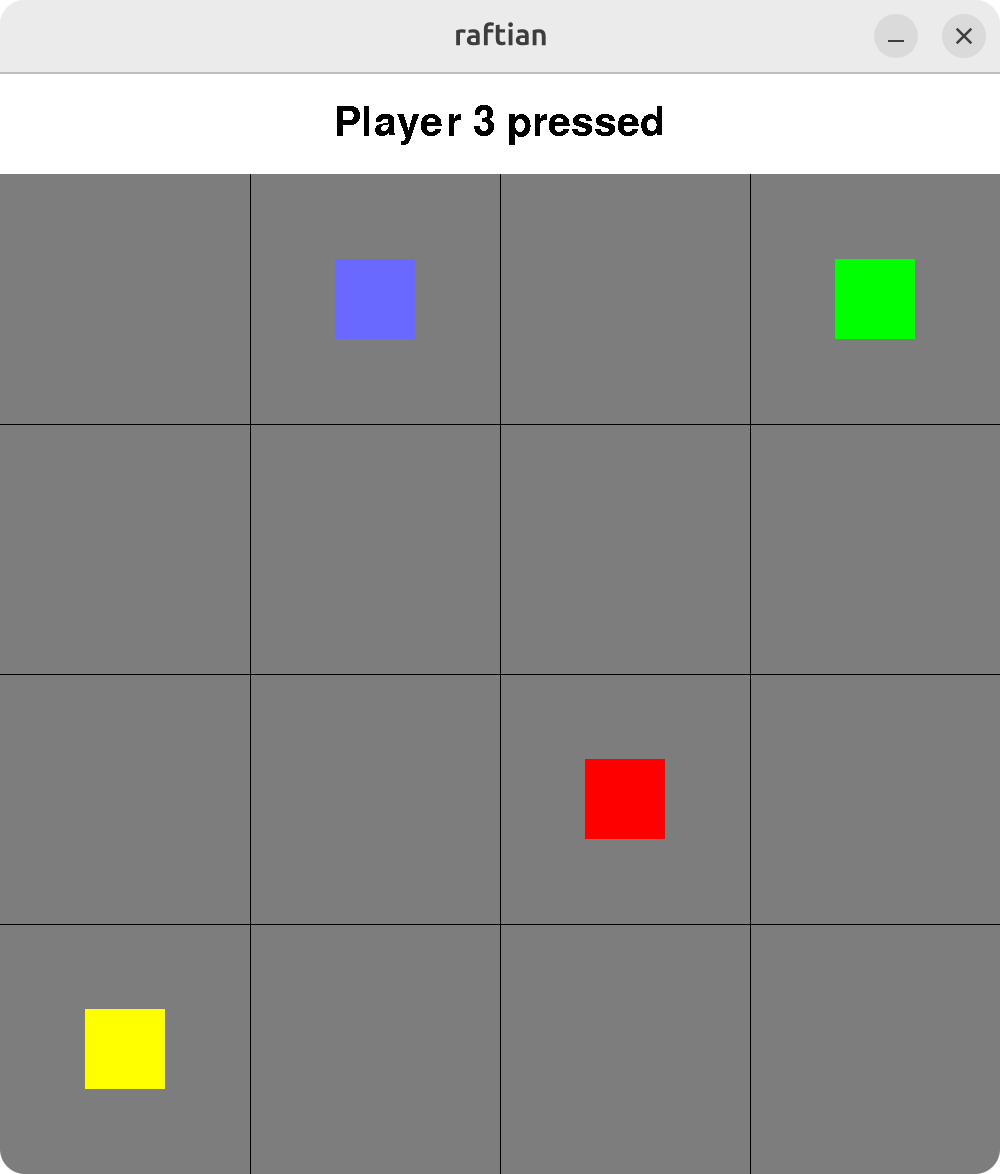
\includegraphics[width=\linewidth]{images/raftian4.png}
        \caption{Player 3 is left with forty HP}
    \end{subfigure}
    \hfill
    \begin{subfigure}{0.31\textwidth}
        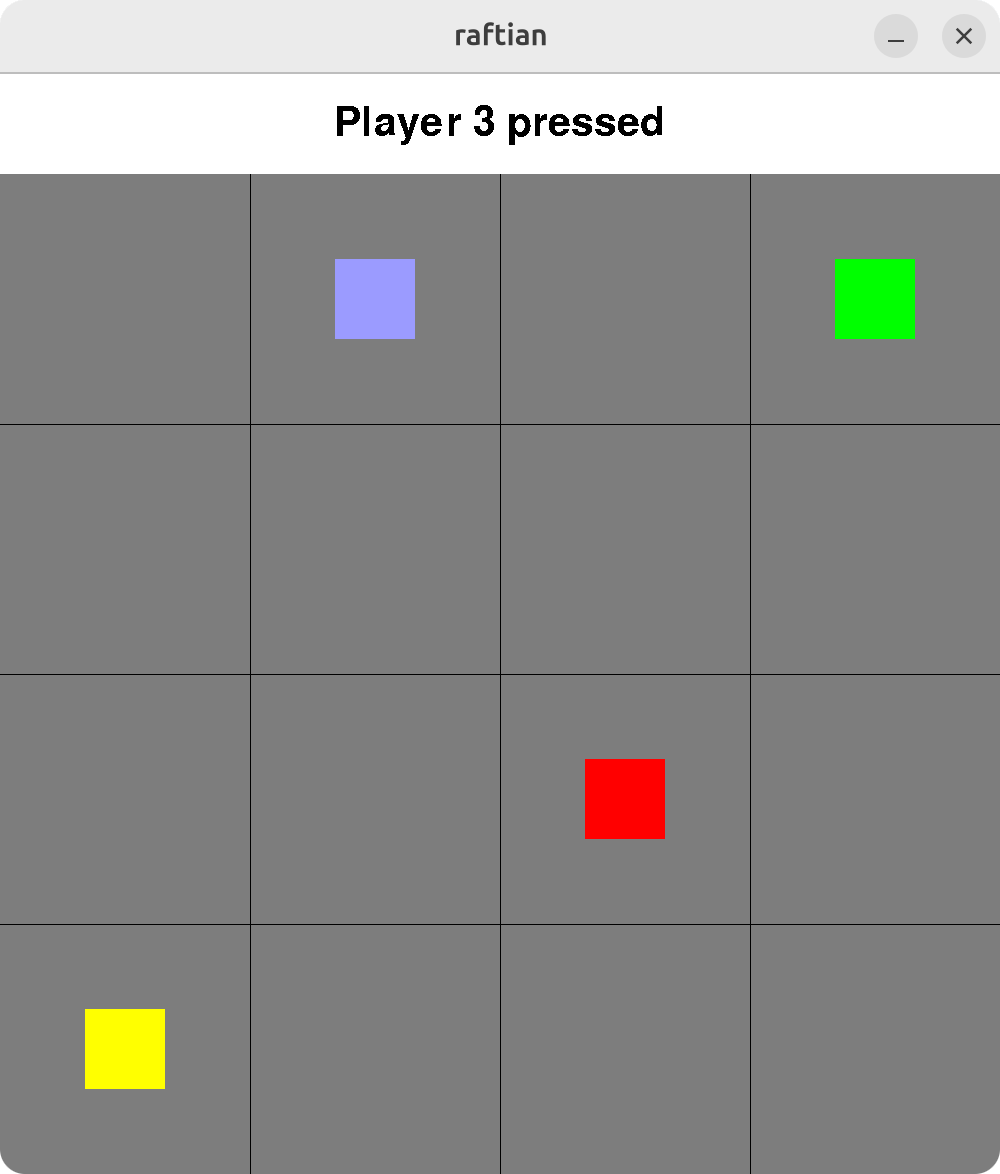
\includegraphics[width=\linewidth]{images/raftian5.png}
        \caption{Player 3 is left with ten HP}
    \end{subfigure}
    \hfill
    \begin{subfigure}{0.31\textwidth}
        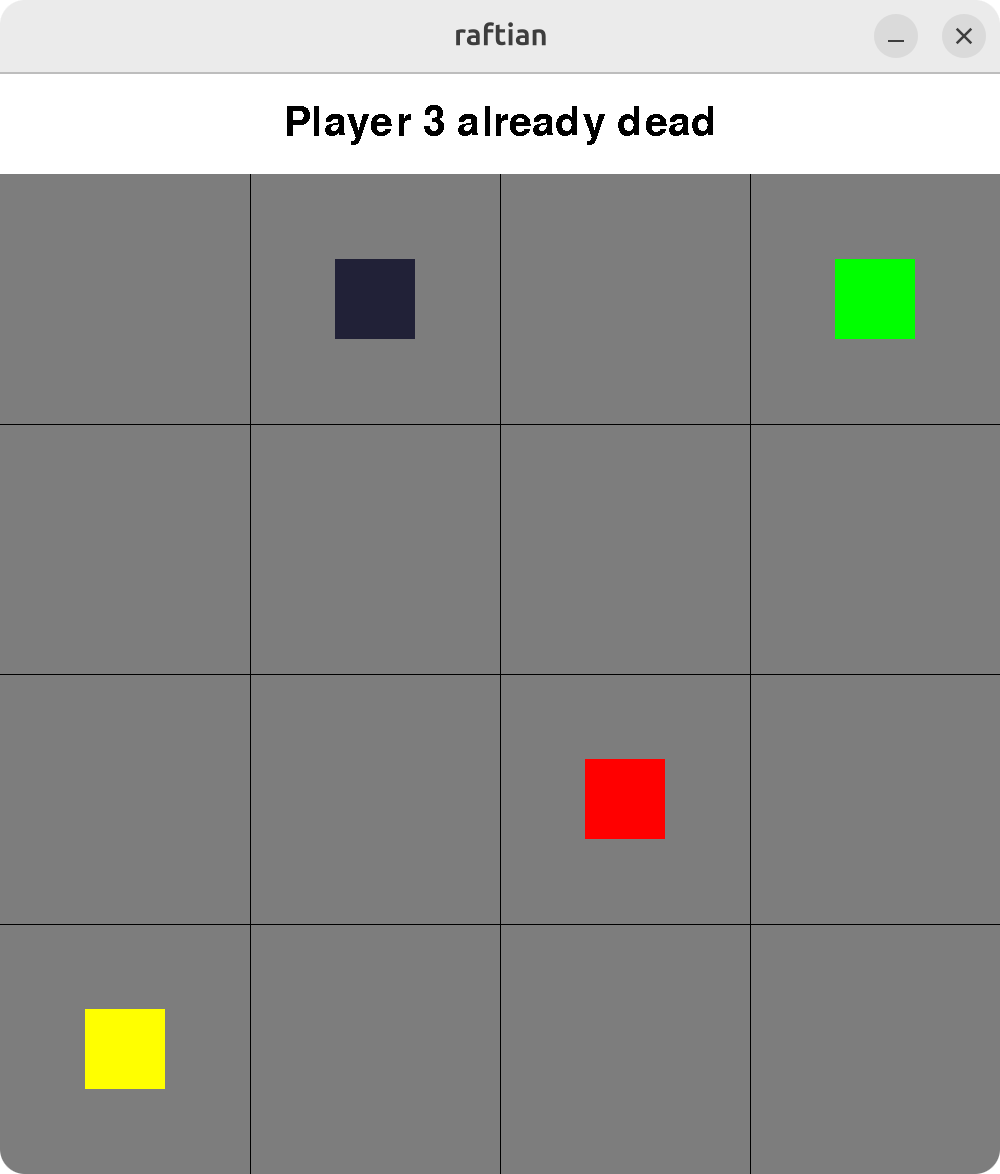
\includegraphics[width=\linewidth]{images/raftian7.png}
        \caption{Player 3 cannot be attacked again}
    \end{subfigure}

    \caption{Different phases of a normal Raftian's game session, Player 3 keeps getting damaged until it dies}
    \Description{Six figures that shows a Raftian game instace in 6 different game phases.}
    \label{fig:raftianUI}
\end{figure}

\subsection{Raftian Node Architecture}

The architecture of a Raftian node can be seen at figure \ref{fig:raftianArch}. Let's explain it: first of all, the game loop and the server are encapsulated in two functions to be handed over to two different threads, enabling concurrent execution (listing \ref{code:startMainThreads}). Whenever a player clicks on (i.e., attacks) one of the four players, the game engine does not apply damage immediately. Instead, it generates a \textit{command} which represent, if we want, the \textit{intention} of attacking said player. This \textit{command} is thus appended to a queue called \textit{pygame\_commands}, one of the two synchronized queues necessary to allow communication between server and Pygame's threads (listing \ref{code:queues}). Both are instances of Python's standard library queue module\footnote{Python's queue, a synchronized queue class: \url{https://docs.python.org/3/library/queue.html}}, which implements thread-safe, multi-producer, multi-consumer queues. 

At this point, Pygame does not concern itself anymore with said user input. The server, by itself, periodically checks the \textit{pygame\_commands} queue (as in listing \ref{code:addCommands}) and, when not empty, removes elements from it (as in listing \ref{code:translateCommands}) and propagates them as entries to the Leader (or to the whole cluster if said server \textit{is} the Leader, as in listing \ref{code:leaderPropagateEntries}).

Then, the Leader propagates to the whole cluster the commands received, which we will now call \textit{orders}. Each server add received orders to its own log, as explained in section \ref{sec:logReplication}, so that they can later be appended to the \textit{raft\_orders} queue when entries get applied to state (as in section \ref{sec:applyToState}). This way, the original user input gets propagated back to the server that generated it in the first place.

Finally, Pygame checks (periodically) the \textit{raft\_orders} queue for orders. When it finds them, it removes them from the queue and updates the user interface accordingly (an example can be seen at listing \ref{code:updateUI}).

The whole idea is to keep server and game engine as separated as possible: the former reads commands, propagates them and writes received orders, the latter reads orders, updates the UI, and writes commands, following a unidirectional cyclic communication pattern.

\begin{python}[label={code:startMainThreads}, caption={Start both Pygame and server's threads}]
def handle_pygame():
    pygame.init()
    #...
    While True:
         #...
def handle_server():
    with Raft(...) as server:
        #...
        server.serve_forever()

server_thread = threading.Thread(target=handle_server)
server_thread.start()
pygame_thread = threading.Thread(target=handle_pygame)
pygame_thread.start()
\end{python}

\begin{python}[label={code:queues}, caption={Queues for commands and orders, they allow inter-thread communication}]
# user inputs trough Pygame which writes them here
# Raft reads them and propagate them to the cluster
pygame_commands = Queue()

# commands that have been applied to state are written here by Raft
# Pygame reads them and update UI accordingly 
raft_orders = Queue()
\end{python}

\begin{python}[label={code:updateUI}, caption={Pygame periodically checks whether there are new orders and updates the UI accordingly}]
while True: # Pygame's main loop
    #...
    while not raft_orders.empty():
        order: Raft.Entry = raft_orders.get()

        for player in players:
            if player.id == order.command and player.hp > 0:
                player.hp -= 30  # apply damage to player:
                #...
\end{python}

\begin{figure}[h]
  \centering
  \includegraphics[width=\linewidth]{images/nodeArchitecture.png}
  
  \caption{Raftian node architecture.}
  \Description{Fiure showing the architecture of a Raftian node, by showcasin how all different component work between each other.}
  \label{fig:raftianArch}
\end{figure}

